\documentclass[defense.tex]{subfiles}
\begin{document}



%-----------------------------------------------------------------------------
% References
%-----------------------------------------------------------------------------

\section{Annex FacNet}

\begin{frame}{Related works}

\begin{itemize}\itemsep2em
	\item \cite{Giryes2016}: Propose the inexact projected gradient descent and conjecture that LISTA accelerate the LASSO resolution by learning the sparsity pattern of the input distribution.
	\item \cite{xin2016maximal}: Study the Hard-thresholding Algorithm and its
	capacity to recover the support of a sparse vector.\\
	The paper relax the RIP conditions for the dictionary.
\end{itemize}
	
\end{frame}


\begin{frame}{Learned FISTA}
The same ideas can also be applied to FISTA to obtain similar procedures:
\begin{figure}[t]
    \centering
	\inputTikZ{.75}{lifsta_tikz.tex}
    \label{fig:ista}
    \caption{Network architecture for L-FISTA.}
\end{figure}
\end{frame}


\begin{frame}{PASCAL 08}

\begin{columns}[T]
\column{.49\textwidth}
\vskip2em
Sparse coding for the PASCAL 08 datasets over the Haar wavelets family.\\[2em]

The sparse coding is performed for patches of size $8\times8$.\\[.5em]
Train over 500 images and test over 100 images.
\column{.49\textwidth}
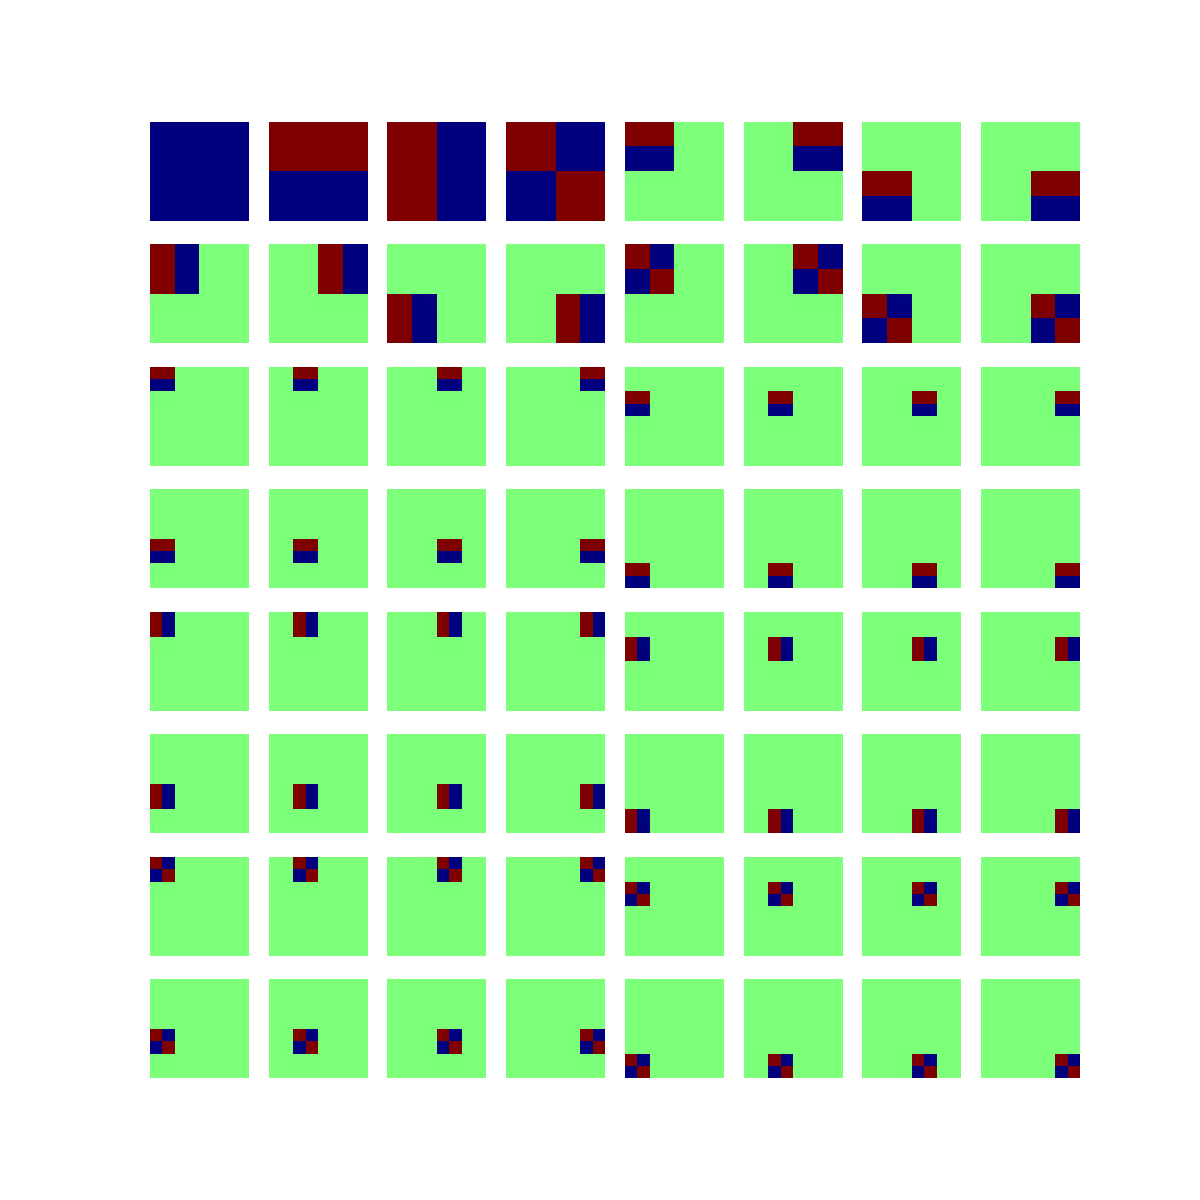
\includegraphics[width=\textwidth]{Wavelets}
	
\end{columns}
	
\end{frame}
\begin{frame}[noframenumbering]{PASCAL 08}
    \centering
    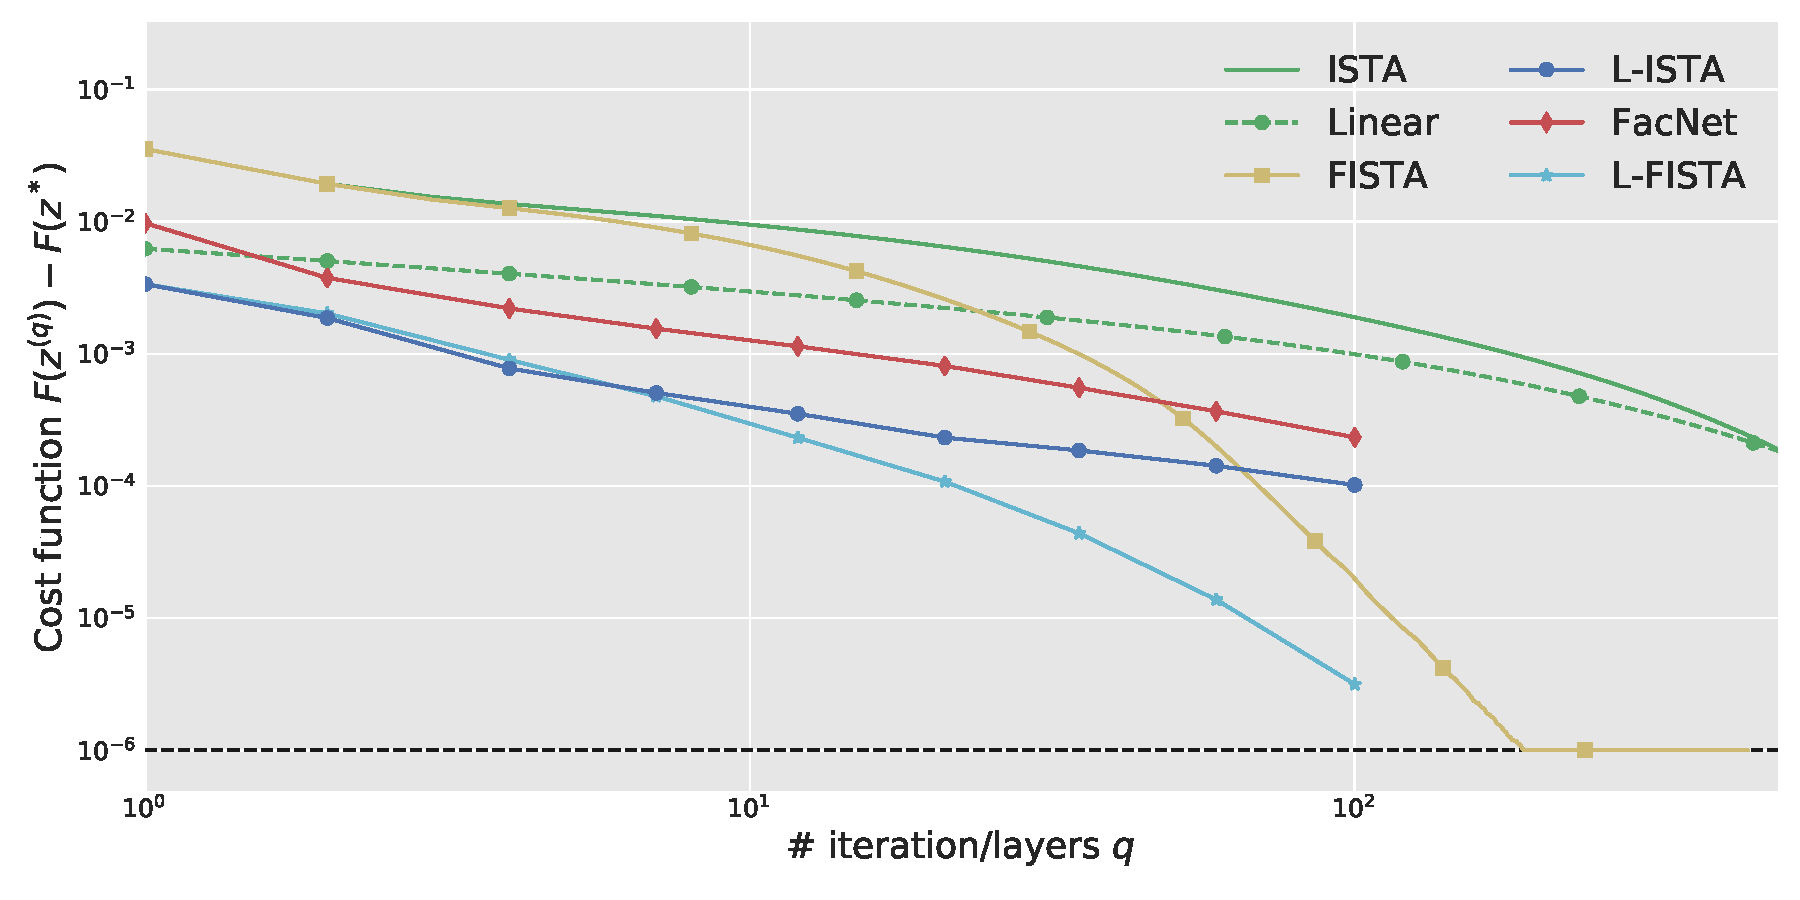
\includegraphics[width=.8\textwidth]{curve_images_seaborn}\\
     Evolution of the cost function $F(z^{(q)})-F(z^*)$ with the number of layers or the number of iteration $q$ for Pascal VOC 2008.
\end{frame}


\begin{frame}{MNIST}
	Dictionary $D$ with $K=100$ atoms learned on 10 000 MNIST samples (17x17) with dictionary learning.
	LISTA trained with MNIST training set and tested on MNIST test set.

    \centering
    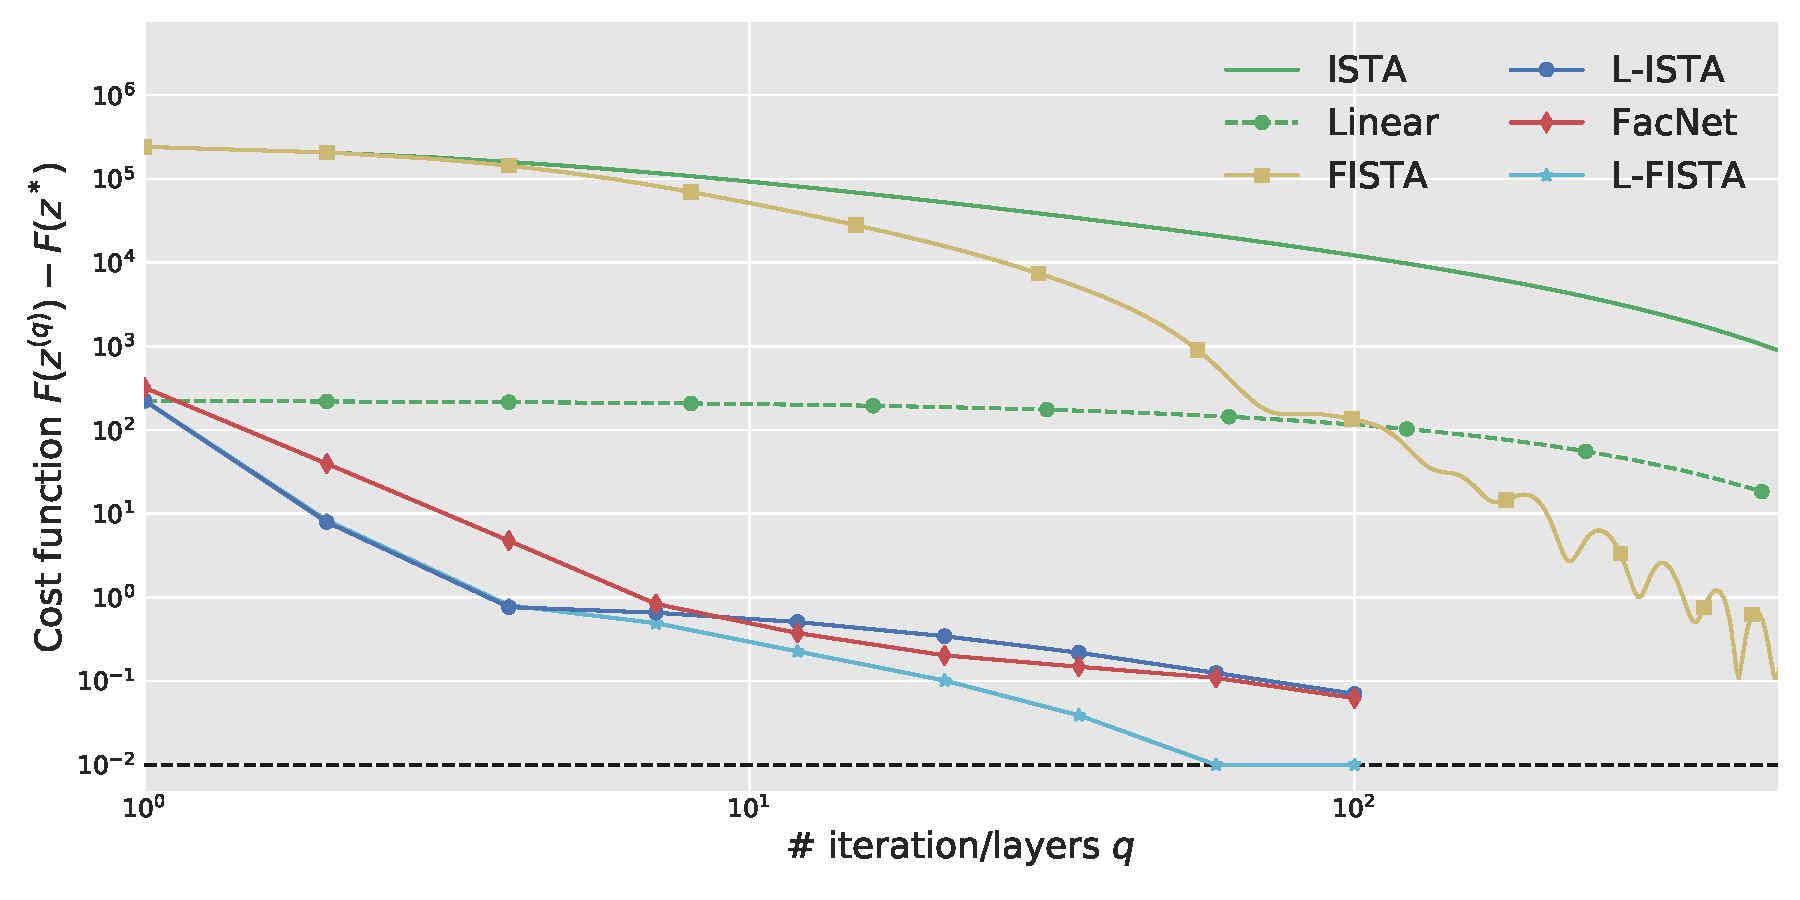
\includegraphics[width=.8\textwidth]{curve_mnist_seaborn}\\
     Evolution of the cost function $F(z^{(q)})-F(z^*)$ with the number of layers or the number of iteration $q$ for MNIST.
\end{frame}

\section{Annex DICOD}

\begin{frame}{Finishing the process in a linear grid?}
	Non trivial point: {\bf How to decide that the algorithm has converged?}\\[2em]
	
	\begin{itemize}\itemsep2em\itemindent1em
		\item Neighbors paused is not enough!
		\item Define a master 0 and send probes.\\
			\hskip3em Wait for $M$ probes return.
		\item Uses the notion of message queue and network flow.\\
			\hskip3emMaybe we can have better way?
	\end{itemize}
	
	
\end{frame}



\section{Singular Spectrum Analysis (SSA)}

\begin{frame}{Singular Spectrum Analysis (SSA) \mycite{Vautard1989}}
\large
	\begin{columns}[T]
		\column{.47\textwidth}
		{\bf Idea}\\[1em]
		\begin{itemize}
			\item Choose a window size $K$ and extract sub series,
			\item Reconstruct a low rank estimate of all the $K$-length sub series,
			\item Decomposition of the series as a sum of "low rank" components.
		\end{itemize}
		\column{.47\textwidth}
		{\usebeamercolor[bg]{itemize}.}\vskip2em
		\begin{itemize}\itemsep1em
		\item[$\rightarrow$] K-trajectory matrix $\pmb X^{(K)}$
		\item[$\rightarrow$] Singular Value decomposition
		$X^{(K)} = \sum_{k=1}^K \lambda_k U_kV_k^T$
		\item[$\rightarrow$] Average along anti-diagonals
	\end{itemize}
	\end{columns}
	\vskip2em
	\begin{columns}[T]
		\column{.9\textwidth}
	
		\begin{itemize}
			\item[$\Rightarrow$] Extract components linked to trend and oscillations
			%\hskip-2em{\bf Issues}
			%\item[$\bullet$] Same pattern present in different low rank components
			%\item[$\bullet$] Representation is "dense", no localization
		\end{itemize}
	
	\end{columns}
\end{frame}



\begin{frame}{Singular Spectrum Analysis}
\large
	We show in the thesis that this solves the following problem

\vskip.6em
\begin{block}{Optimization problem}
Solve a convolutional list square
\begin{equation}\label{eq:sparse_code}
	Z^*, \pmb D^* = \arg\min_{Z, \pmb D} \frac{1}{2} \left\|X - \sum_{k=1}^K z_k*D_k\right\|_2^2,
\end{equation}
with constraints $\langle D_i, D_j \rangle = \delta_{i, j}$ 
\end{block}

\vskip1em
\begin{itemize}
	\item $\pmb D$ is the dictionary with $K$ patterns in $\mathbb R$ of length $W$
	\item $Z$ is an activation signal, or coding signal in $\mathbb R^K$ of length $L = T-W+1$
\end{itemize}
\end{frame}



\begin{frame}{Toward a sparse representation}
\Large
	{\bf Issues}\\[1em]
	\begin{itemize}\itemsep1em
	\item[] Same pattern present in different low rank components
	\item[] Representation is "dense", no localization
	\item[] Different representation for each signal
	\end{itemize}

\end{frame}



\section{Post-training for Deep Learning}
\label{sec:post_train}


\begin{frame}{Post-training for Deep Learning}

	{\bf Paper with J. Audiffren: } arxiv:1611.04499\\[2em]

	Use the idea to split the representation learning and the task resolution:\\[1em]
	\begin{itemize}\itemindent1em\itemsep1.5em
		\item \underline{{\it Post-training} step:} only train the last layer,
		\item \underline{Easy problem:} this problem is often convex,
		\item \underline{Link with kernel:} close form solution for optimal last layer.
		\item \underline{Experiments:} consistent performance boost with multiple architecture.
	\end{itemize}
	
\end{frame}

% section post_train (end)

\end{document}